\section{背景与定义}
\subsection{背景---访问模式与数据安全\cite{ref0,ref00}}\par
随着云计算、云服务的发展,越来越多的数据被存储在云端服务器上。然而,一旦服务器遭到恶意攻击,或者不可信的云服务提供商恶意获取服务器信息,用户的隐私信息就会泄露。传统的手段是对数据内容进行加密,密钥由用户个人持有.用户通过上传、下载密文数据来保护个人的隐私信息不被泄露。\par
然而,加密只能保证数据内容的机密性,由于CPU与内存之间的内存总线 (Address Bus) 是无法加密的,攻击者通过客户端访问的数据块地址序列(访问模式),依旧能够推断出其它的隐私信息。如文献\cite{ref1}中,攻击者可以通过搜集访问模式,可以通过统计的手段推断出80\%已加密的搜索请求。而在逆向工程领域\cite{ref2,ref3},内存地址的访问模式可以帮助攻击者分析出程序的结构,例如,在程序运行的过程中,攻击者可以观察到对内存位置100,101,X(102或103),104重复出现,他就可以推断出这是一个包含着条件分支的循环。
\begin{figure}[H]
    \centering
    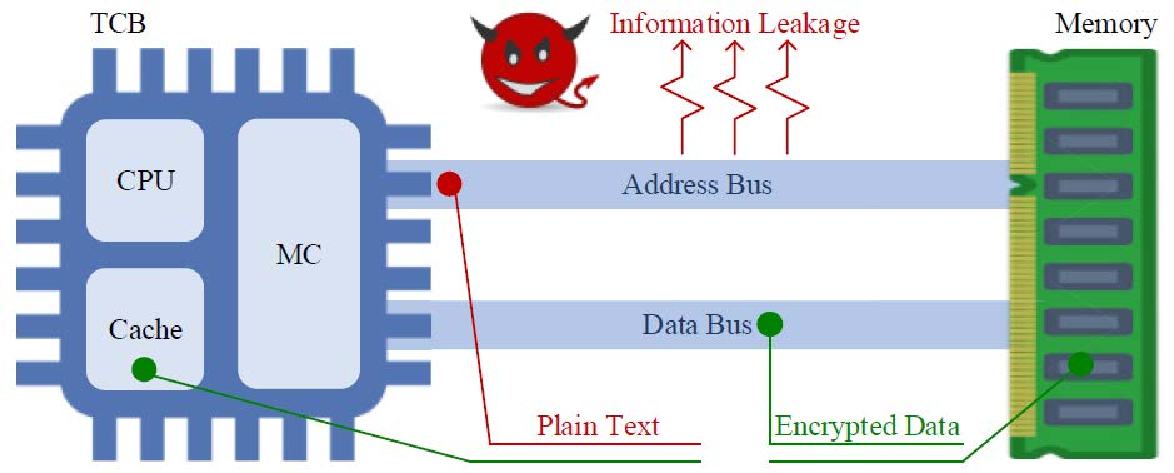
\includegraphics[width=0.8\textwidth]{introduction/leakage.pdf}
    \caption{内存总线上访问模式的泄露}
    \label{fig:leak}
\end{figure}
Goldreich与Ostrovsky在论文中\cite{ref4}提出了不经意随机访问机 (Oblivious RAM, abbr. ORAM)技术。这一技术的目的是隐藏对真实数据块的访问,使得攻击者不能区分每一次访问是真实的还是随机的。不经意随机访问机应用于云存储系统可以有效的防止攻击者利用访问模式获取隐私信息,减小数据存储系统的攻击面,打破了单纯使用传统加密方式来保护数据隐私的系统框架,为用户提供更完善的安全存储服务。\par%
但是,不经意随机访问机也会带来额外的开销,比如:为了隐藏访问模式,需要对多个数据块进行访问,这增大了客户端与服务器之间的带宽,客户端需要更大的缓存空间来存储从服务器端返回的额外数据块。所以,不经意随机访问机的实用性还面临很大的挑战。
\subsection{ORAM安全性定义}\par
为保护和混淆内存的访问模式,ORAM 保证了在存储器中的任意数据块不会永久驻留在某一个物理地址中,这确保了任意两次访问不会产生关联。同时,ORAM将每一次读写访问 (access) 细化成一次读取加一次写回的原子操作 (operation) ,其中读问转化成读取内容再写回相同内容,写访问转化成读取内容再写回更新后的内容,使得攻击者不能够区分具体的访问方式。ORAM能很好地保护
\begin{enumerate}
    \item 访问数据块的位置
    \item 数据块请求的顺序
    \item 对相同数据块的访问频率
    \item 具体的读写访问方式
\end{enumerate}
\par\noindent 下面我们对ORAM的安全性进行正式的定义:
\begin{definition}\textbf{ORAM安全性}
    \newline
    设$\vec{y}$为长度为$M$的一系列数据操作序列,$\vec{y}=(op_1,id_1,block_1),\ldots,(op_M,id_M,block_M)$,$op_i$为读操作$read(id_i)$,其读取标识符为$id_i$的块;或写操作$write(id_i,block_i)$,将新数据$block_i$写入到标识符为$id_i$的块中。如果$op_i=read(id_i)$,那么$block_i=null$。
    \newline
    给定操作序列$\vec{y}$,设其经过ORAM加密后的访问模式为$A(\vec{y})$,该ORAM体制是安全的当期仅当对任意两个相同长度序列$\vec{y}, \vec{y'}$,其访问模式$A(\vec{y}), A(\vec{y'})$计算上不可区分。
\end{definition}\par
为了让读写操作不可区分,标准的解决方案是始终采用“先读后写”的操作,不需要写入的时候通过写入无效信息 (dummy write) 来进行混淆。
\subsection{发展脉络}
不经意随机访问机的概念最早起源于RAM (random access machine)模型,RAM是一种重要的计算仿真手段。在这个模型中,处理器通过对存储器的读写来实现程序的执行。上个世纪80年代,为了隐藏程序对内存的访问模式来避免软件的逆向工程,Goldriche等人在此基础上提出了ORAM\cite{ref2},开启了ORAM的研究历程。不经意随机访问机面临的最大问题是性能开销大。纵观不经意随机访问机的发展。其设计模型大致可以分为5类:简单模型、平方根模型\cite{ref5,ref6}、层次模型\cite{ref5}、分区模型\cite{ref7}和树状模型\cite{ref8,ref9}。不同的设计模型表示服务器存储数据块的数据结构不同,用户通过对服务器ORAM的访问来获取所需的数据块,这些模型设计的目标主要还是提高性能。本文主要介绍后4种模型及其变种,并简介ORAM的最新研究进展。